\chapter{开发环境的配置}
\label{cha:Environment}

在这一章,着重阐述Windows 10环境下开发环境的配置方法。

\section{Mega 2560开发环境}


\section{ESP 32开发环境配置}

\subsection{Windows平台ESP-IDF工具链的标准设置}

ESP-IDF 需要安装一些必备工具,才能围绕 ESP32 构建固件,包括 Python、Git、交叉编译器、menuconfig 工具、CMake和 Ninja 编译工具等。

要安装 ESP-IDF 必备工具,最简易的方式是下载 ESP-IDF 工具安装器\footnote{\url{https://dl.espressif.com/dl/esp-idf-tools-setup-2.2.exe}}。

安装器可安装所需的交叉编译器、OpenOCD、cmake 和 Ninja 编译工具,以及一款 mconf-idf 配置工具。此外,本安装器还可在有需要时下载、运行 Python 3.7 和 Git For Windows 的安装器,如图~\ref{fig:IDF-Installer}。

\begin{figure}[htbp]
    \centering
    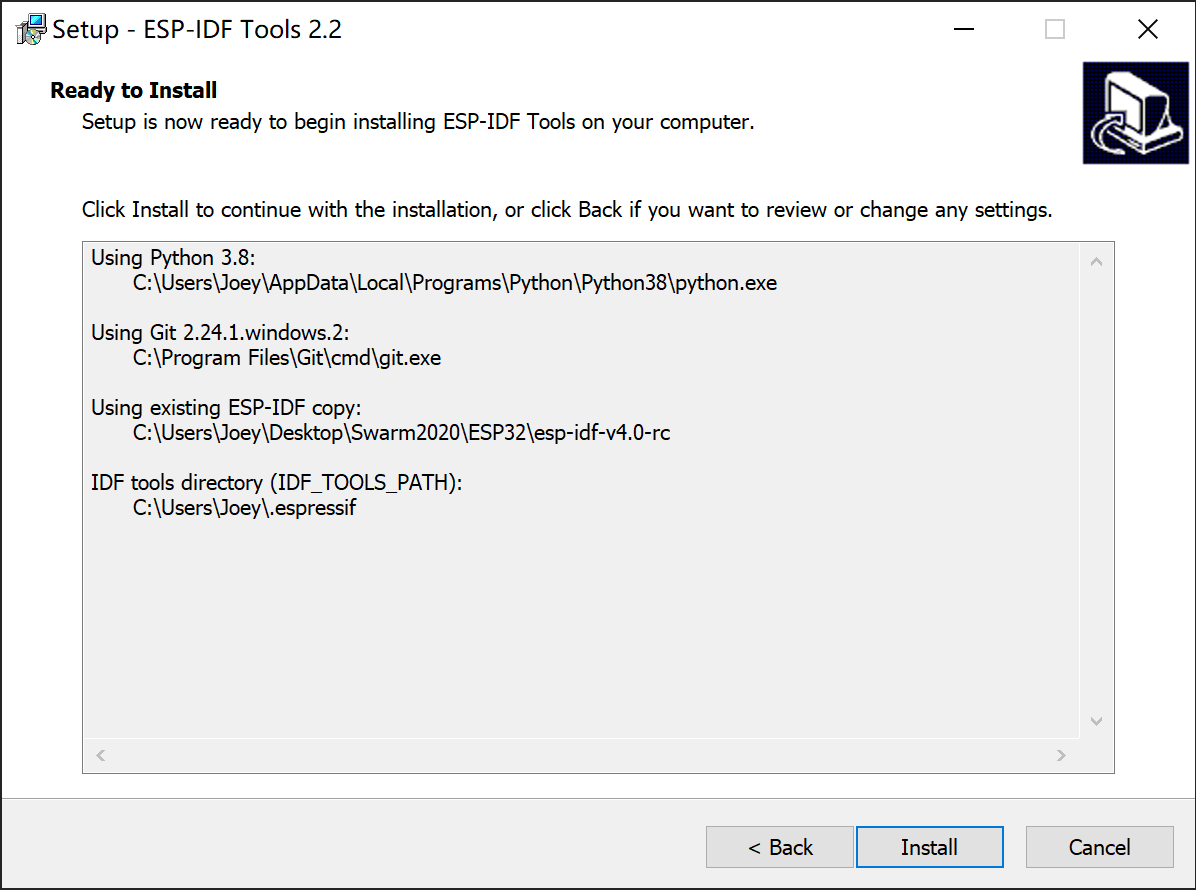
\includegraphics[width=0.7\columnwidth]{IDF-Installer.png}
    \caption{ESP-IDF 工具安装器配置}
    \label{fig:IDF-Installer}
\end{figure}

\subsection{获取 ESP-IDF}

除了工具链,您还需要供 ESP32 使用的 API(软件库和源代码),具体请见 ESP-IDF 仓库。

请将 ESP-IDF 下载到您的本地。

获取本地副本:打开终端,切换到你要存放 ESP-IDF 的工作目录,使用 \mintinline{powershell}|git clone| 命令克隆远程仓库:

% \mint{powershell}|git clone -b v4.0-rc --recursive https://github.com/espressif/esp-idf.git|


GitHub 中”下载 zip 文档”的功能不适用于 ESP-IDF,所以需要使用 git clone 命令。作为备份,可以在没有安装 Git 的环境中下载 Stable version 的 zip 归档文件。直接在\url{https://github.com/espressif/esp-idf/releases/download/v4.0-rc/esp-idf-v4.0-rc.zip}下载并解压。

\subsection{安装 Python 软件包}

ESP-IDF 所需的 Python 软件包位于 IDF-PATH/requirements.txt 中。您可以运行以下命令进行安装:

\mint{powershell}|python -m pip install --user -r $IDFPATH/requirements.txt|

\begin{tcolorbox}
    This is my first \textbf{tcolorbox}.
\end{tcolorbox}

\subsection{开始创建工程}

现在,您可以开始准备开发 ESP32 应用程序了。您可以从 ESP-IDF 中 examples 目录下的 get-started/hello-world 工程开始。ESP-IDF 编译系统不支持带有空格的路径,可能需要复制到其他目录下再运行。

\subsection{连接设备}

现在,请将您的 ESP32 开发板连接到 PC,并查看开发板使用的串口。

通常,串口在不同操作系统下显示的名称有所不同:

\begin{itemize}
    \item Windows 操作系统: COM1 等
    \item Linux 操作系统: 以 /dev/tty 开始
    \item MacOS 操作系统: 以 /dev/cu. 开始
\end{itemize}


\subsection{工程配置}